\chapter{Results}
% Preliminary investigation and results
\begin{figure*}[t]
 \begin{center}
\subfloat[Google maps\label{subfig:gmap}]{ 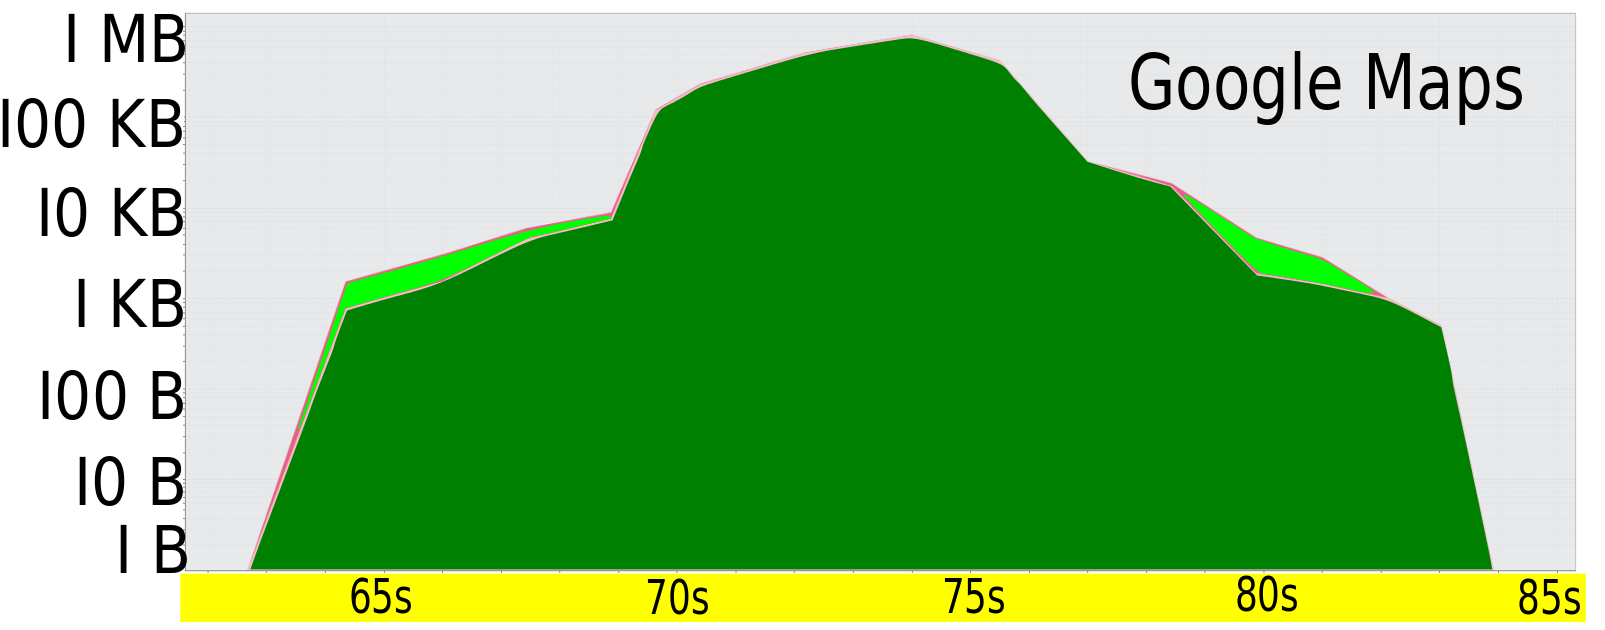
\includegraphics[scale=0.15]{Figures/gmapgps60to80c.png}}
\subfloat[YouTube\label{subfig:ytube}]{ 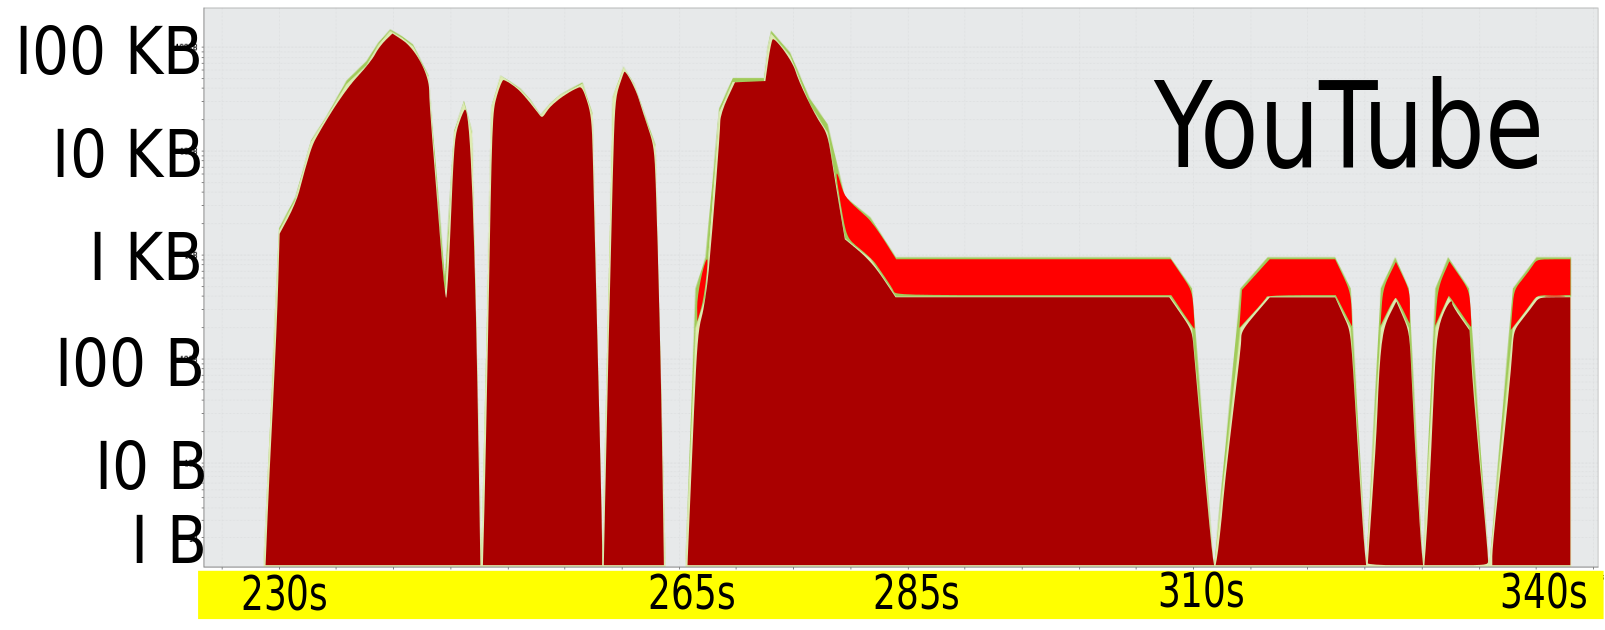
\includegraphics[scale=0.15]{Figures/Youtube230c.png}}
 \end{center}
 \caption{Randomly profiled data usage patterns}
 \label{fig:TrepnDataUsage}
\end{figure*} 
Smart-phone is a system-on-chip architecture with three key components  \emph{Application processor} to handle user applications, \emph{Modem processor} to handle transmission and reception and \emph{Peripheral devices(I/O)} to interact with users. In smart-phones, power consumption of any I/O component is sometime higher than the power consumption of the CPU or at the least comparable. In \cite{EModel} the problems and flaws in the power models derived from external power meters and those derived from (hardware) utilization-based well explained by considering the types of components having \textit{tail power states},  not having quantitative utilization(e.g. camera on/off) and system calls that change power states but not mean any utilization of hardware. As system calls are the only way for application can use I/O components, system call based power modelling is better one. Thus Energy profiling with all its overheads is the very important first step.
\subsection{Power states,logging and semantic data}
The Advanced Configuration and Power Interface(ACPI) specification has been evolving as a de-facto common hardware interfaces in Operating System-directed configuration and  Power Management(OSPM) for both devices and entire systems. When profiling either an individual application or entire platform it is useful to fetch information about the states of system, device and processors, as in table \ref{table:states}, so that better decision can be made to achieve energy efficiency. We are currently using Qualcomm's Trepn Profiler \cite{trepn}. We study the behaviours of the system and applications running in the system including CPUs usage, memory usage, data usage. 
\begin{table}[h]
\begin{tabular}{|l|l|l|}
\hline
Global System States & Device Power States  & Processor Power States \\
\hline
G0 Working & D0 - Fully-On  & C0\\
G1 Sleeping & D1  & C1\\
G2/S5 Soft Off & D2 & C2\\
G3 Mechanical Off & D3hot & C3\\
& D3 - Off & \\
\hline
\end{tabular}
\caption{ACPI/OSPM defined power states}
\label{table:states}
\end{table}

As data communication is one of the main reasons for the quicker energy drain in the smart-phones, it is interesting example to profile the data usage patterns of the different applications. In figure \ref{fig:TrepnDataUsage}, profiled data usage patterns of two applications, namely, \textit{Google Maps} and \textit{YouTube} is shown. While profiling google maps, GPS was turned ON at 20th second, maps were zoomed-in and then the device is navigated in random direction. We observed as shown in figure \ref{subfig:gmap}, sudden high usage of data occurred about 10 seconds in the time interval [70, 80]. In this manual profiling and inspection, it is inferred that action of zooming-in the map is the reason for high data usage. Does the state of the GPS being ON has any effect on data usage? The answer seems \emph{no} because of the fact that the GPS is turned ON at 20th second already. If the device lay in the fixed position, the above question doesn't make sense. If the device is in navigation, then it requires fine-tuned profiling again. While profiling youtube, a video is randomly picked for playing, after few seconds the screen is rotated to play the video in full screen mode, the video is continued to play. We observed as shown in figure \ref{subfig:ytube}, the initial aggressive data communications due to pre-fetching. 
These scenario implies: 
\begin{itemize}
\item Usage of resources such as CPU, Memory, GPU and Data varies with respect to applications
\item Weighted effect on energy usage with respected to the resources should be studied
\item Fine-grained profiling is data-intensive and computations-intensive
\item Profiler should be self-energy efficient
\item Automation of profiling with added semantics is extremely challenging
\item Detailed study of interdependencies and contexts is required
\item Mobile cloud computing is suitable
\end{itemize}

We are developing R computing language configured cloud application \emph{EnergyApp} to develop and test energy models and visualize the insights on sample data. The application right now manually let the user to inspect the data collected by Trepn profiler. It also shows simple interactive plots where one can compare the parameters for example, as CPU usage against memory usage for the applications. We further investigate with statistical data analysis and machine learning algorithms. Then we model the smart-phones as dynamic systems as in control systems to develop self-controllers for the participating systems. Then set of data preprocessing methods will be implemented. Then knowledge graph building process will take place. After this phase assembling orchestration will take place. 
\subsection{Future Work}
Orchestrator is in essence the behaviour predictor of the participating devices with respect to time, location and as many as added contexts. The agent application installed in the smart-phones which report logs to the orchestrator will be facilitated with local validator and action triggers which is regularly updated by orchestrator according to the needs to avoid wasting orchestrator energy and data communication for well learnt case. In order to successfully deploy such orchestration service, we need to study and explore all its components defined in the previous section and their interdependencies in detail.  Then we focus on the questions including 1) how to develop low energy consuming profiler? 2) how to reduce logs reporting thus by reduce data communication? 3) how to make orchestrator an epic predictor of device behaviours? 4) how to find optimal responsibilities of local agent by ensuring minimal computation ans resources? 5) Is it best fit for mass open source contribution? 6) What are the de-facto tools for over all implementation? We plan to implement and test the prototype iteratively. This work could be then extended or simplified to other type of IoT devices.





%https://en.wikipedia.org/wiki/Advanced_Configuration_and_Power_Interface
%The data is produced either by collecting real data by participatory sensing or by simulation in case of limited availability of real data or in case of testing. 

% Excesss ---- %

%From a power management perspective, OSPM/ACPI promotes the concept that systems should conserve
%energy by transitioning unused devices into lower power states including placing the entire system in a low-power state (sleeping state) when possible.

%\State $syslog \gets \{err, data\}$

%
%Control theory concept to be explained by considering smartphones as dynamic systems( applications and processes = linear/non-linear time/frequency domain signals )
%The above fig is demo, final version may change
%\begin{algorithm}                      % enter the algorithm environment
%\caption{Generating Energy Efficient Decision Signals }          % give the algorithm a caption
%\label{alg1}                           % and a label for \ref{} commands later in the document
%\begin{algorithmic}                    % enter the algorithmic environment
%	\Procedure{EnableEnergyEfficiency}{}
%    \REQUIRE System-call logs
%    \ENSURE Energy Efficient Decision Signals
%    \STATE $syslog \Leftarrow \{err:\{\}, data:\{\}\}$ % $\#h$
%    \IF{$n < 0$}
%        \STATE $X \Leftarrow 1 / x$
%        \STATE $N \Leftarrow -n$
%    \ELSE
%        \STATE $X \Leftarrow x$
%        \STATE $N \Leftarrow n$
%    \ENDIF
%    \WHILE{$N \neq 0$}
%        \IF{$N$ is even}
%            \STATE $X \Leftarrow X \times X$
%            \STATE $N \Leftarrow N / 2$
%        \ELSE[$N$ is odd]
%            \STATE $y \Leftarrow y \times X$
%            \STATE $N \Leftarrow N - 1$
%        \ENDIF
%    \ENDWHILE
%    \EndProcedure
%\end{algorithmic}
%\end{algorithm}

%\State $i \gets \textit{patlen}$
%\BState \emph{top}:
%\If {$i > \textit{stringlen}$} \Return false
%\EndIf
%\State $j \gets \textit{patlen}$
%\BState \emph{loop}:
%\If {$\textit{string}(i) = \textit{path}(j)$}
%\State $j \gets j-1$.
%\State $i \gets i-1$.
%\State \textbf{goto} \emph{loop}.
%\State \textbf{close};
%\EndIf
%\State $i \gets i+\max(\textit{delta}_1(\textit{string}(i)),\textit{delta}_2(j))$.
%\State \textbf{goto} \emph{top}.
%
%\Procedure{Init}{init}
%\State $err \gets \{\}$
%\State $data \gets \{\}$
%\EndProcedure


%\begin{algorithm}
%\caption{Generating Energy Efficient Decision Signals}\label{eeeff}
%\begin{algorithmic}
%\Require System-call logs
%\Ensure Energy Efficient Decision Signals
%
%\MVAt Devices
%\Procedure{RegisterRequest}{device\_id}
%\EndProcedure
%
%\Procedure{SendLogAndError}{device\_id,err,data}
%\EndProcedure
%
%\MVAt Orchestrator
%\Procedure{RegisterDevice}{device\_id}
%\EndProcedure
%
%\Procedure{EnableEnergyEfficiency}{}
%%\State $syslog \gets \{err, data\}$
%\EndProcedure
%
%\end{algorithmic}
%\end{algorithm}



%\subsection{Inside the control box}
%discussion about 1)Time vs Frequency Domain signals 2) Laplace/ Fourier Transforms 
%\subsection{Data analysis}
%Find the categories and interested questions


%\begin{figure}[H]
% \begin{center}
% 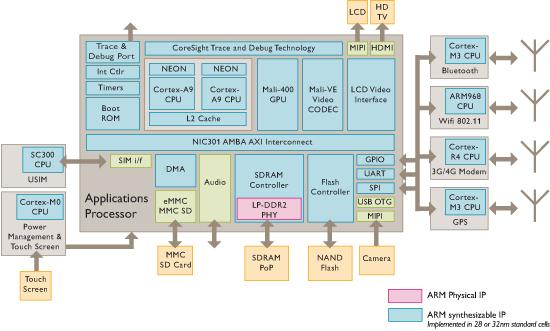
\includegraphics[scale=0.45]{Figures/mobilearch1.png}
% \end{center}
% \caption{ARM Architecture(courtesy:www.arm.com)}
%\end{figure} 